\begin{figure}[t!]
\eightpoint
\begin{verbatim}
float->float filter FIR (float sampRate, int N) {
    float[N] weights;

    init {
        weights = calcImpulseResponse(sampRate, N);
    }

    prework push N-1 pop 0 peek N {
        for (int i=1; i<N; i++) {
            push(doFIR(i));
        }
    }

    work push 1 pop 1 peek N {
        push(doFIR(N));
        pop();
    }

    float doFIR(int k) {
        float val = 0;
        for (int i=0; i<k; i++) {
            val += weights[i] * peek(k-i-1);
        }
        return val;
    }

    handler changeWeights(float[N] newWeights) {
        weights = newWeights;
    }
}
\end{verbatim}

\begin{minipage}{2.8in}
\begin{verbatim}
float->float pipeline Main {
  add Source();  // code for Source not shown
  add FIR();
  add Output();  // code for Output not shown
}
\end{verbatim}
\end{minipage}
\begin{minipage}{0.5in}
\vspace{-12pt}
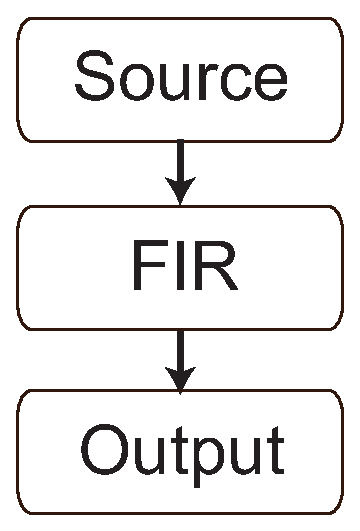
\psfig{file=fir-pipeline,width=0.5in}
\end{minipage}
\vspace{-6pt}
\caption{Example StreamIt program with FIR filter.\protect\label{fig:fir-pipeline}}
\vspace{-6pt}
\end{figure}

\section{The StreamIt Language}

StreamIt is an architecture-independent language for high-perfor-mance
stream programming~\cite{thies-cc02}.  The compiler is publicly
available~\cite{streamitweb} and includes backends for multicore
architectures, clusters of workstations, and the MIT Raw architecture.

The model of computation in StreamIt is grounded in (but not limited
to) synchronous dataflow~\cite{lee87}.  In this model, the programmer
implements independent actors, or {\it filters}, which translate data
items from input channels to output channels.  Filters are composed
into graphs that represent the overall computation.  The key property
of synchronous dataflow is that the number of items consumed and
produced during each execution of a filter is known at compile time,
allowing the compiler to perform static scheduling and optimization.
StreamIt also allows filters to declare a dynamic data rate, which
requires the support of a runtime system.

An example StreamIt program appears in Figure~\ref{fig:fir-pipeline}.
It is based on an FIR filter, which contains three stages of
execution.  The most important is the {\it work} function, which
represents the steady-state execution step and is called repeatedly by
the runtime system.  Within the work function, a filter may {\it peek}
at a given element on the input tape, {\it pop} an item off the input
tape, or {\it push} an item to the output tape.  The total number of
items peeked, popped, and pushed are declared as part of the work
function.  Note that if the peek rate exceeds the pop rate, it
represents a sliding window computation in which some input elements
are accessed across multiple invocations of the filter.

In addition to the work function, a filter may declare an {\it init}
function to initialize internal data structures, as well as a {\it
  prework} function to perform specialized processing of data items
prior to the steady state.  The prework function is needed in cases
where the initial processing has a different input or output rate than
the steady-state processing.

As depicted in Figure~\ref{fig:structures}, StreamIt provides three
hierarchical primitives for composing filters into stream graphs.  A
{\it pipeline} represents a sequential composition of streams, in
which the output of one stream feeds into the input of the next.  A
{\it splitjoin} represents a parallel set of streams, which divulge
from a common {\it splitter} and converge to a common {\it joiner}.
The types of splitters and joiners are predefined by the StreamIt
language; they encompass duplication and weighted round-robin
behaviors.  Finally, a {\it feedbackloop} represents a cycle in the
stream graph.

\enlargethispage*{12pt}

Because pipelines, splitjoins, and feedbackloops are all single-input
and single-output, they can be hierarchically composed.  By analogy to
structured control flow, we designate these primitives as {\it
  structured streams}.

In addition to supporting steady-state flows of data, StreamIt also
provides a mechanism for sending out-of-band control information
between actors.  Termed {\it teleport messaging}, this feature allows
filters to deliver messages that are timed with respect to the data
items in the stream, even if they are not embedded in the stream
itself.  For example, a distant filter could invoke the {\it
  changeWeights} handler in the FIR filter in order to adjust the
weights in the filter.  All message senders and message latencies are
known at compile time to avoid non-deterministic outcomes.  Additional
details on teleport messaging are available
elsewhere~\cite{thies-ppopp05}.

\begin{figure}[t!]
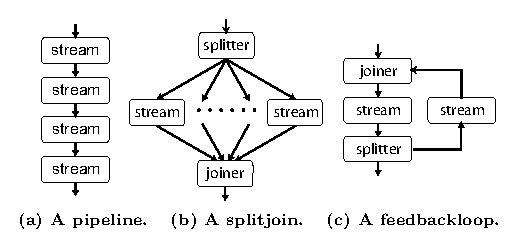
\psfig{file=stream-structures,width=\columnwidth}
\caption{Hierarchical stream structures supported by StreamIt.\protect\label{fig:structures}}
\end{figure}

